%%%%%%%%%%%%%%%%%%%%%%%%%%%%%%%%%%%%%%%
%%% LATEX HEADERS
%%%%%%%%%%%%%%%%%%%%%%%%%%%%%%%%%%%%%%%

\documentclass[11pt]{article}
\usepackage{rotating}                           
\usepackage[dvips]{epsfig}
\usepackage{multirow}
\usepackage{amsfonts,amssymb,amsmath}
\usepackage{array}                      
\usepackage{url}
\usepackage{thumbpdf}
\usepackage{natbib}

\usepackage{vmargin}
\setpapersize{USletter}
\setmarginsrb{1.0in}{1.0in}{1.0in}{1.0in}{0.5in}{0.2in}{0in}{0.2in}
\renewcommand{\baselinestretch}{1.25}

%%%%%%%%%%%%%%%%%%%%%%%%%%%%%%%%%%%%%%%
%%% SHORTCUTS
%%%%%%%%%%%%%%%%%%%%%%%%%%%%%%%%%%%%%%%


%%%%%%%
%%% Vignette Headers
%%%%%%%

%\VignetteIndexEntry{accuracy}
%\VignetteKeywords{statistical computing}                                       
%\VignetteVersion{1.0}
%\VignetteTitle{Tools For Accurate and Reliable Statistical Computing}


%%%%%%%%%%%%%%%%%%%%%%%%%%%%%%%%%%%%%%%
%%% DOCUMENT HEADERS
%%%%%%%%%%%%%%%%%%%%%%%%%%%%%%%%%%%%%%%

\let\code=\texttt
\let\proglang=\textsf
\newcommand{\pkg}[1]{{\normalfont\fontseries{b}\selectfont #1}}


%%%%%%%%%%%%%%%%%%%%%%%%%%%%%%%%%%%%%%%
%%% DOCUMENT STARTS
%%%%%%%%%%%%%%%%%%%%%%%%%%%%%%%%%%%%%%%

\usepackage{Sweave}
\begin{document}


\section{NOTE}

This vignette is based on:
``accuracy: Tools for Accurate and Reliable Statistical Computing'' by
Micah Atman, Jeff Gill, Michael P. McDonald, in the \emph{Journal of Statistical Software}, Vol. 21, Issue 1, Jul 2007.

Please use the above article for citation and reference purposes.

\section{Introduction}

Social science data are often subject to measurement error, and nearly all methods of statistical 
computing can yield inaccurate results under some combinations of data and model specification. 
This is an issue of practical concern -- since our previous work and that of others, demonstrates 
that published analyses are affected with surprising frequency \citep{AltGilMcD03,AltGilMcD05,MccVin99, AltMcD02,AltMcD03}. Unfortunately, most practitioners ignore even routine numerical issues 
in statistical computing. This is in contrast to some scientific and engineering disciplines, 
which require assessments of the accuracy of both data and 
	results.\footnote{For example, publication in any of the American Institute of Aeronautics 
	and Astronautics journals requires that all reported data must be accompanied with error 
	bars, and the numerical accuracy of the resulting analyses be explicitly assessed \citep{AIAA98}.}

A simple example (below), using generated data, shows how numeric issues can affect even seemingly 
simple calculations. Consider the calculation of a variable's dispersion: In \proglang{R}, the function 
\code{sd} returns the `sample standard deviation', but does not provide an option to return the
`population standard 
	deviation'.\footnote{The population standard deviation differs from the sample standared 
	deviation in that it uses $n$ rather than $n-1$ as a divisor.} 
The three functions below compute this quantity. The first two functions are direct implementations 
of textbook formulas, and the third simply adjusts the results of the \emph{sd} function.

\vbox{
\begin{Schunk}
\begin{Sinput}
> sdp.formula1 <- function(x) {
+     n <- length(x)
+     sqrt(n * sum(x^2) - sum(x)^2)/n
+ }
> sdp.formula2 <- function(x) {
+     sum(sqrt((x - sum(x)/length(x))^2))/length(x)
+ }
> sdp.formula3 <- function(x) {
+     sqrt(var(x) * (length(x) - 1)/length(x))
+ }
\end{Sinput}
\end{Schunk}
}

To see the damaging effects of numerical errors, we apply these functions to the following 
generated data frames, each of which produces columns of numbers, of increasing magnitude, 
that have standard deviations of 0.5.

\vbox{
\begin{Schunk}
\begin{Sinput}
> testMat <- function(len = 50, digits = c(3, 5, 7, 9, 11, 13, 
+     15, 17, 19)) {
+     len <- 2 * len
+     dat <- NULL
+     for (i in digits) {
+         dat <- as.data.frame(cbind(dat, 1:len%%2 + 10^i))
+     }
+     names(dat) <- as.character(digits)
+     return(dat)
+ }
\end{Sinput}
\end{Schunk}
}

Although the three formulas for calculating the standard deviation of the populations are \emph{mathematically} correct, the results computed with them are obviously wrong. The first method is particularly bad: The range of inputs that yield correct answers is much smaller
for the first method than for the others, some of the errors produced by the first method are 
extremely large, and the pattern of errors is not easily discernable as the 
number of observations in each column increases. 

\vbox{
\begin{Schunk}
\begin{Sinput}
> dat <- testMat(4)
> print(rbind(sapply(dat, sdp.formula1), sapply(dat, sdp.formula2), 
+     sapply(dat, sdp.formula3)), digits = 3)
\end{Sinput}
\begin{Soutput}
       3   5   7   9  11  13  15 17 19
[1,] 0.5 0.5 0.5 0.0 0.0 0.0 0.0  0  0
[2,] 0.5 0.5 0.5 0.5 0.5 0.5 0.5  0  0
[3,] 0.5 0.5 0.5 0.5 0.5 0.5 0.5  0  0
\end{Soutput}
\end{Schunk}
}
\vbox{
\begin{Schunk}
\begin{Sinput}
> dat <- testMat(10)
> print(rbind(sapply(dat, sdp.formula1), sapply(dat, sdp.formula2), 
+     sapply(dat, sdp.formula3)), digits = 3)
\end{Sinput}
\begin{Soutput}
       3   5    7   9  11  13       15  17  19
[1,] 0.5 0.5 0.51 NaN 0.0 0.0 1.34e+07 NaN NaN
[2,] 0.5 0.5 0.50 0.5 0.5 0.5 5.00e-01   0   0
[3,] 0.5 0.5 0.50 0.5 0.5 0.5 5.00e-01   0   0
\end{Soutput}
\end{Schunk}
}
\vbox{
\begin{Schunk}
\begin{Sinput}
> dat <- testMat(50)
> print(rbind(sapply(dat, sdp.formula1), sapply(dat, sdp.formula2), 
+     sapply(dat, sdp.formula3)), digits = 3)
\end{Sinput}
\begin{Soutput}
       3   5     7   9  11  13  15 17 19
[1,] 0.5 0.5 0.493 0.0 0.0 0.0 0.0  0  0
[2,] 0.5 0.5 0.500 0.5 0.5 0.5 0.5  0  0
[3,] 0.5 0.5 0.500 0.5 0.5 0.5 0.5  0  0
\end{Soutput}
\end{Schunk}
}

The second and third of the methods are much better -- they produce correct results for the test 
data, up to the 8th column, and yield simply zero 
	thereafter.\footnote{In \proglang{S-PLUS}, \code{colStdevs(x,unbiased=F)}, yields results 
	identical to formula's 2 and 3.} In fact, in this example, the second and third \code{sdp} 
	formulas are accurate, and it is the test inputs that suffer from roundoff error -- as 
	$1 + 10^{16}$ silently rounds to $10^{16}$.
 
When social scientists encounter similar behavior from software, they often find it baffling. Ironically, 
as user-friendly statistical packages have enabled social scientists to adopt increasingly sophisticated 
statistical methods, users have become even less familiar with the computational details involved in their 
	estimation.\footnote{This is probably exacerbated by the fact that most social scientists do not 
	write software -- and as \citep{Stromberg04} points out, many academics (incorrectly) perceive writing 
	statistical software for public use (and particularly for robust methods) to be unrewarding.} 
We have demonstrated such issues to numerous colleagues, and most consider it entirely mysterious until the 
underlying mechanics have been thoroughly explained. These comments, collected by one reviewer or our 
previous work \citep{VanZandt05} after showing a version of the standard deviation example 
to his colleagues, are representative: 
\begin{quote}
	I polled my colleagues, all quantitative psychologists who routinely perform complex 
	statistical analyses by showing them (a similar table of standard deviations, as computed 
	by \proglang{Excel}). The responses I got ranged from ``I don't want to hear about this,'' 
	and ``Oh my God!'' to ``I'm confused.'' Colleagues of a certain age, those who remember 
	punching Fortran code onto cards or tape, were not surprised at all. Another colleague 
	said ``These issues are completely unknown to us.''.
\end{quote}
Our example is relatively easy to grasp because it uses simple calculations on a restricted range of inputs. 
In practice, the computational issues involved are more complex, and inaccurate results less obvious to users. 
Many computational problems reveal themselves only as obscure warning messages delivered at the end of 
analysis, or not as all, yielding purportedly correct estimates. The various sources of computational 
accuracies can include: un-modeled measurement error; bugs; errors in data input; data that is ill-conditioned 
for a particular model; floating point underflow, overflow, and rounding; non-random structure in ``random'' 
number generators; local optima or discontinuities in optimization landscapes; inappropriate or unlucky 
choices of starting values; and inadequate stopping criteria. 

A number of book-length works are devoted to each of these sources of error, and correcting them may require 
intensive examination of the numerical details of a particular problem. Fortunately, a number of 
relatively straightforward techniques exist to \emph{detect} such problems. While these techniques cannot 
prevent or fix errors, they can alert the researcher to many situations in which numerical and measurement 
errors would otherwise lead an analysis astray. 
 
We describe here a set of software tools we have developed to make these techniques 
readily available to users of the \proglang{S} language. In particular, we have created \pkg{accuracy},
 a package that runs in \proglang{R}  
\citep{R07} and \proglang{S-PLUS}, to help researchers to
determine whether the results of their statistical analyses are potentially affected by measurement and 
numerical error. This package provides a variety of numerical tools for improving 
the accuracy and reliability of statistical analysis, including: methods to compare the
results from multiple models, sensitivity analyses for numerical and measurement error,
 methods for checking whether a local optima has ``trapped'' a maximum likelihood estimate, 
non-linear regression, or other optimization-based method; a routine to supply \emph{true} random 
numbers by tapping external physical sources of entropy; and a generalized Cholesky method for 
recovering information from non-invertible Hessians. The \pkg{accuracy} module also provides an interface 
to \pkg{Zelig}, a package for \proglang{R} that provides a simple unified way to estimate, 
interpret, and present the results of a large range of statistical methods 
\citep{Zelig07}.\footnote{In this article we discuss \pkg{accuracy} version 1.28. This article 
	was written using \code{Sweave} \citep{Leisch02}, which ensures that what appears in the article corresponds 
	precisely to the output for that version. We continue to improve the package and to release future 
	versions. Thus the output in the current version of accuracy may differ slightly from our examples 
	here.}
  
\section{Common Sources of Inaccuracy}

\subsection{Accuracy and stability}
What is \emph{computational accuracy}? The computational accuracy of a statistical analysis can be thought of 
as the distance (using a well-behaved measure) between the actual results produced by the computer program and results that would have been produced had all algorithms been
implemented correctly, and all calculations been performed perfectly. 
 
Computational accuracy alone is not enough to ensure reliable computations. Given infinitely precise and accurate inputs, a computation can yield perfectly accurate results, and yet the same program yield wildly incorrect answers in the presence of minute amounts of measurement or rounding
error in the inputs. Since, in practice, data is almost certainly subject to some finite measurement error, and calculations to some finite numerical error, reliable statistical computations must be \emph{computationally stable} as well as accurate.

Somewhat more formally, stability is simply the distance of the true estimate, given the data, Y, from the computer output, given the data and noise:
\begin{equation}
    S = \nabla \left(estimate\left(Y\right), output\left(Y+\Delta\right)\right)
\end{equation}
Less formally, a stable algorithm gives, to quote \citet{Higham02}, ``almost the right answer to almost the same problem.''
 
Instability may arise from or be exacerbated by several levels of problems: accumulated numerical errors in the computations used to implement the model; limitations in the algorithms guiding these computations; or interactions between the form of the statistical model with the data being analyzed. Regardless of the source of problem, if the data inputs are not given with absolute precision and accuracy, whether because of
measurement error in collecting the data or numerical error in processing it, and if the model estimation process is unstable, then any inferences follow are unlikely to be correct.
 
To understand how to detect and correct for computational problems, it is useful to understand their sources. Most statistical models, most problems at the \emph{computational} level fall into three broad categories: First, computational problems occur because nearly all software uses floating-point number representations for computation rather than using perfect symbolic representation. Second, computational problems occur because of the limits or incorrect use of optimization algorithms. Third, computational result from non-randomness in ``random'' number generation.

\subsection{Floating point arithmetic errors} 
A floating point numbering system is a subset of the real number system where elements have the form: 
$y=\pm m \times \beta ^{e-t}$. Each numbering system is characterized by the following quantities: a 
base $\left( \beta \right) $, an exponent range $\left( e,e_{\min } \leq e\leq e_{\max } \right) $, a
\index{precision}precision $\left( t\right)$, a sign, and a mantissa $\left(m,0\leq m\leq \beta^{t}-1\right)$.
For a particular \emph{y} only \emph{m}, \emph{e}, and a sign are stored. In IEEE floating point,
which is now used in almost all software, one can think of each number as being represented, in base 2, 
a single bit for the sign, a sequence of $t$ bits for the mantissa, and an exponent of length $e$ 
	bits.\footnote{There are some additional complexities involved with ``sub-normal'' numbers, 
	infinite values, and the precise details of how rounding and other errors are handled during 
	computation. See \citet{Overton01} for a detailed description of the IEEE floating point standard.}

Unfortunately, some numbers cannot be exactly represented using this scheme. An interesting example 
is the number $0.1$, which is an infinitely repeating decimal in base 2. 
 \emph{Rounding} error occurs when this number is represented as a floating point value,
 since $0.1$ must be represented in a finite number of bits: ${\rm 0}{\rm .000110011}\overline {{\rm 0011}}\ldots$
Moreover, floating point arithmetic is not necessarily exact even when the operands happen to be represented exactly. For example, 
when floating point numbers are added or subtracted their exponents must first be normalized: The 
mantissa of the smaller number is divided in two while increasing its exponent, until the two 
operands have the same exponent. This division may cause low-order bits in the mantissa of the 
smaller number to be lost, which results in rounding error. In addition, floating point 
operations are susceptible to overflow and to underflow, when a number is larger (smaller) than the 
largest (smallest) number capable of being represented. (Careful programmers can avoid some
 of these problems, with considerable effort, by explicit use of multiple precision arithmetic 
 through packages such as \pkg{gmp} \citep{gmp07}. Most functions and calculations in \proglang{R}, \proglang{S-PLUS},
 and other statistical languages, however, remain potentially susceptible.) 

As \citet[page 229]{Knuth97} points out, one of consequences of the inaccuracies in floating point 
arithmetic is that the associative law of arithmetic sometimes breaks 
	down:\footnote{Where $\oplus$ denotes the standard arithmetic operators.}
\begin{equation}
    \left( a\oplus b\right) \oplus c\neq a\oplus \left( b\oplus c\right)
\end{equation}

 Also, as \citet[Section 2.10]{Higham02} 
notes, limits on precision can interfere with the mathematical properties of functions. Although 
many elementary functions can be efficiently calculated to any desired degree of precision, the 
necessity of returning the final results at a fixed precision leads to situations in which the 
computed function may not have all of the mathematical properties of the true function of interest. 
The requirements of preserving symmetries, mathematical relations and identities, and correct 
rounding to the destination precision can conflict, even for elementary functions.

\subsection{Non-linear optimization errors} 
The effects of numerical and measurement error can both interact and accumulate. In the standard 
deviation examples above, rounding error had a large cumulative effect on the final result. As another example, in 
linear regression, when several explanatory variables are near-collinear, their individual parameter estimates are based on little information, and are thus less stable, to measurement errors. The cumulative effects of numerical error are, however, more often 
visible in non-linear estimations. And the accuracy of many non-linear estimates
is, in addition, \emph{inherently} dependent on well-informed (or fortuitous)
choice of computational methods and parameters that are not included in the formal statistical model, 
such as: starting values, convergence tolerances, iteration step sizes, and optimization algorithms. 

Standard techniques for the optimization of likelihood functions (and other non-linear modeling 
techniques) typically involve the following steps: 
\begin{enumerate}
	\item	Choose (implicitly or explicitly) starting values for each parameter in the model.
	\item	Use analytic gradients (or numerically calculated differences) of the 
		likelihood function, given the current parameter values, to determine a 
		``direction'' to move. 
	\item Identify an appropriate step size.
	\item	Take a ``step'' in that direction, updating the parameter values accordingly.
	\item	Update the parameters accordingly in accordance with the step size and direction.
\end{enumerate}
Steps two through five are repeated until the algorithm has converged to a stationary 
point, or some other stopping criterion (such as a limit on the number of iterations) is satisfied. 

Floating point errors can affect the process of nonlinear optimization by inducing discontinuities 
in the optimization function or its gradients, and optimization algorithms sometimes converge to 
such false optima. As \citet{ChaiTrav04a} point out, the classical 
theory of singularities breaks down under floating point arithmetic -- 
pseudo-singularities (induced by computational inexactness) form a generic set rather 
than a set of measure zero. 

In addition, even without numerical error, non-linear models may be ill-conditioned with respect 
to a particular dataset, and the estimates thus particularly sensitive to errors in variables. Finally, 
unless the optimization surface is convex or unimodal, no computationally-tractable optimization 
algorithm, even without error in variables or calculation, is \emph{guaranteed} to converge to a 
global optimum in a finite amount of time. Thus, when there are multiple local optima, the resulting parameter estimates will be incorrect unless the starting values chosen are within the basin of attraction of the global optimum.


\section{Comparing model results}

Because of the potential for computational and other errors, it is sometimes necessary to systematically compare two tables of output that purport to estimate the same statistical model using the same data. \pkg{accuracy} provides a number
 of functions, introduced in version 1.19, to aid in these comparisons. These tools 
 are meant to be used when comparing results of statistical benchmarks to output
already known to be correct; when moving to a new version of
a statistical package; or when building an extension to an existing model. In each of these cases one may want to verify that the new algorithm or implementation yields the same results as an alternative. 

Model comparisons may also be used as a component of robustness testing, to check whether a change in computational parameters 
(such as starting values) or implementations lead to different results. 

The simplest function, \code{LRE()}, computes the \emph{log relative error} between 
two numbers (or vectors, matrices, or arrays). This is roughly interpretable
as the number of significant digits of agreement between the first and second sets
of numbers, with larger numbers indicating closer agreement. An LRE value of 16 is the
maximum achievable using standard IEEE double precision -- and thus indicates complete 
agreement within the standard storage precision of \proglang{R} and \proglang{S-PLUS}.
Numbers less than or equal to zero indicate complete disagreement between two numbers.

 
To illustrate the use of the LRE function, we compare the output of the function for the student 
\emph{t} distribution to numerically correct benchmark 
	output.\footnote{This benchmark output was computed using two independent algorithms, 
	using multiple precision arithmetic, for more details see Altman, Gill and McDonald 2003, 
	Section 3.2.5.} 
First we compute the quantiles, by applying the \code{qt} function to the probability values 
given in the test data:

\vbox{

\begin{Schunk}
\begin{Sinput}
R> data("ttst")
R> tqt <- qt(ttst$p, ttst$df)
\end{Sinput}
\end{Schunk}

The \code{LRE} function is invoked to compare the computed quantiles to the
correct quantiles, which are contained in another column of the benchmark data. 
This produces a table that shows how many of the 10,000 \code{qt} evaluations
tested were accurate to a given number of 'digits': from 0 (totally inaccurate) to 16 (as accurate as the benchmark can measure):

\begin{Schunk}
\begin{Sinput}
R> lrq <- LRE(tqt, ttst$invt)
R> table(round(lrq))
\end{Sinput}
\begin{Soutput}
   4    5    6    7    8    9   10   16 
   6  138 5180 1897  173   20    2   36 
\end{Soutput}
\end{Schunk}
}

The function \code{modelsCompare} can be used to compare the results from 
a list of two or more models. Its default behavior is to extract the 
estimated coefficient values from the model summary, 
 compare these sets of coefficients using the 
\code{LRE} function, and report for each coefficient the largest of the differences 
between the first model given and
each of the subsequent models in the list. (If, for example one is interested only in
both parameter estimates and standard errors, one can use other
functions to select the parameters of interest for use in \code{modelsCompare}.) For example, we can
use \code{modelsCompare} to see to what extent the use of \code{mle} optimization methods 
to solve the same problem affects the estimated parameter coefficients:

First, run the models separately.
\begin{Schunk}
\begin{Sinput}
R> library("stats4")
R> x <- 0:10
R> y <- c(26, 17, 13, 12, 20, 5, 9, 8, 5, 4, 8)
R> ll <- function(ymax = 15, xhalf = 6) -sum(stats::dpois(y, lambda = ymax/(1 + 
+     x/xhalf), log = TRUE))
R> fit1 <- mle(ll)
R> fit2 <- mle(ll, method = "Nelder-Mead")
R> fit3 <- mle(ll, method = "CG")
R> fit4 <- mle(ll, method = "SANN")
R> fit5 <- mle(ll, method = "L-BFGS-B")
\end{Sinput}
\end{Schunk}

Then use \code{modelsCompare} to generate a report on the list of models.

\begin{Schunk}
\begin{Sinput}
R> modelsCompare(list(fit1, fit2, fit3, fit4, fit5), param.function = modelBetas)
\end{Sinput}
\begin{Soutput}
    ymax    xhalf 
1.568974 1.374715 
\end{Soutput}
\end{Schunk}


We have also supplied a convenience function, \code{modelsAgree}, which uses \code{modelsCompare} to provide a simple logical test that two models agree
to a given number of digits for all coefficients. For example, the following lines
 be used in ``if'' expressions to test that selected models agree to two 
 significant digits:                                 

\begin{Schunk}
\begin{Sinput}
R> (min(as.vector(modelsCompare(list(fit1, 
+     fit2), param.function = function(x) coef(summary(x))))) >= 
+     2)
\end{Sinput}
\begin{Soutput}
[1] TRUE
\end{Soutput}
\begin{Sinput}
R> modelsAgree(fit1, fit2, digits = 2, param.function = modelBetas)
\end{Sinput}
\begin{Soutput}
[1] TRUE
\end{Soutput}
\end{Schunk}

While \code{modelsCompare} aids in ad hoc comparisons among different implementations of the same model, often a more systematic approach is needed. The next section shows how to use \pkg{accuracy} to systematically compare the results of the same model across slightly perturbed inputs. 

\section{Methods for sensitivity analysis through data perturbation}

A straightforward way to test that a given model is stable with respect to
some forms of numerical and measurement error is 
to repeatedly introduce small random perturbations to the data, on the order of the measurement error of the instruments used to collect it, and then recalculate the estimate. When the range of estimates produced using 
this technique vary greatly the model estimation is necessarily unstable, although
the converse is not necessarily true. Where a model is already known to be statistically appropriate,
this type of sensitivity analysis will give the researcher greater confidence that the their 
results are robust to numerical and measurement error.

Data perturbations were described as a sensitivity test in early work by \citet{BeaRubBar76,BeaRubBar77}, who also developed a stability index based on this idea. Similar methods have been 
recommended by  \citet{GilMurWri81,Pregibon81,Cook86,Belsley91}. 
Belsley's approach evaluates collinearity in linear models regression models by adding random                                                               
disturbances to suspected variables and assessing the consequences for parameter stability, thus
exaggerating subtle effects to make them more detectable. 
\citet{HenBelGrot04} extends Belsley's collinearity diagnostic to models of
categorical variables. In separate work, \citet{ParPieEgg00} formalize a variant of 
numeric perturbations, which they call ``Monte Carlo Arithmetic,'' which replicates an analysis while 
introducing uniformly distributed perturbations (in the form of random rounding) to all values in 
all calculations. Extensive surveys of these methods and others are found in \citet{AltGilMcD03} and in \citet{ChaiTrav04a,ChaiTrav04b}.
Here we discuss the mathematical intuitions behind the general methodology. 

To see how perturbations affect the estimation process,
consider two likelihood functions: a standard form based on the observed data $\ell(\theta,\mathbf{x})$, 
and an identical specification but with perturbed data $\ell_\mathbf{p}(\theta,\mathbf{x}_\mathbf{p})$. 
Here $\mathbf{p}$ denotes an individual perturbation scheme: $\mathbf{p}=[p_1,p_2,\ldots,p_n] \in 
\Re^n$ applied to the data: $\mathbf{x}=[x_1,x_2,\ldots,x_n] \in \Re^n$. One
can show that comparing the two likelihood functions is analogous to comparing an un-weighted 
likelihood function $\ell(\theta,\mathbf{x})=\sum_i\ell_i(\theta,\mathbf{x}_i)$ to a weighted 
version $\ell_\mathbf{p}(\theta,\mathbf{x}_\mathbf{p})=\sum_i p_i \ell_i(\theta,\mathbf{x}_i)$. 

Alternatively, one could define the unperturbed likelihood function to be one in which there are null perturbations 
or weights: $\ell_{\mathbf{p}_0}(\theta,\mathbf{x}_{\mathbf{p}_0})=\sum_ip_{0i}\ell_i(\theta,
\mathbf{x}_i)$, where $\mathbf{p}_0$ is simply a vector of $1$'s. This provides two maximum 
likelihood vectors for comparison: $\hat{\mathbf{\theta}}$ and $\hat{\mathbf{\theta}}_\mathbf{p}$. Our 
approach is to evaluate the range of $\hat{\theta}$ 
produced by multiple samples of $\mathbf{x}_\mathbf{p}$ generated by randomly production of 
$\mathbf{p}$ disturbances across different datasets, $\mathbf{x}$. This builds upon the very 
mechanical approach of \citet{Cook86} who observes maximizing and minimizing perturbations, and 
roughly follows a simpler test of logistic regression given by \citet{Pregibon81}.

Although this evaluation methodology is not restricted to a particular class of likelihood functions,
\citet{Cook86} shows that for ``well-behaved'' functions there is a straightforward mapping between 
perturbations of data and perturbations of the model 
	\footnote{Cook 1986 does not explicitly enumerate these behavioral preconditions, 
	but the analysis used does rely on likelihood functions being twice continuously differentiable.} 
For example, normally-distributed noise added to the data induces a corresponding small mean-shift in 
the likelihood curve \citep{StlCoo93}.

Sensitivity analyses are invaluable because they can applied where benchmark tests and independent 
confirmation are unavailable or inconclusive. Moreover, sensitivity analyses can be applied to the 
actual data under study. Perturbation analyses can serve to draw attention to potential problems 
in an algorithm, implementation, or model.

It is important to note, however, that sensitivity analysis cannot alone demonstrate whether a 
particular set of estimates are correct, nor can they be used to improve estimates of 
``correct'' values. The mean of the range of parameter estimates produced by sensitivity is, in 
fact, likely to be slightly biased -- it is well known that explanatory variable measurement error 
introduces bias (although, as above, this bias is slight and well-behaved, under certain conditions). 
Furthermore, in recognizing the statistical problems with measurement error, we do not advise 
intentionally exacerbating it as an \emph{estimation} technique. Rather, the perturbations are a means of \emph{testing} the 
reliability of the estimates produced by a particular model and set data. 

In summary, perturbation may introduce bias, but if the problem is well-conditioned and the 
algorithm and implementation accurate, the bias should be small. Models that react dramatically to modest levels of measurement error warrant caution. Furthermore, any bias introduced by perturbations should be the same across different implementations of the model, thus perturbations are one means of comparing the relative stability of competing computational approaches to model estimation. 

\subsection{Running sensitivity analysis}
The \pkg{accuracy} package makes perturbation-based sensitivity
 analysis simple to apply and to interpret. For many models, running
 a sensitivity analysis involves only three steps.                             
\begin{enumerate}
\item Specify the data, and model.  
\item Give this specification to \code{sensitivity()} to run.
\item Use \code{summary()} or \code{plot(summary())} to display the sensitivity of the parameter estimates to perturbations.
\end{enumerate}


The \code{sensitivity()} command works automatically almost with any \proglang{R} and \proglang{S-PLUS} model, including: \code{lm}, 
\code{glm}, and \code{nls}. All that is required is for the model to accept a data frame argument, and to returns estimated coefficients through
the standard \code{coef()} interface.

The example below shows how to conduct a sensitivity analysis of the classic 
analysis by using \code{sensitivity()} and default noise

functions. For example, to run a sensitivity analysis, using the classic \citet{Longley67}
dataset, a well-studied example known to have multi-collinearity, execute the following command: 


\vbox{
\begin{Schunk}
\begin{Sinput}
R> plongley <- sensitivity(longley, lm, Employed ~ ., ptb.R = 500)
\end{Sinput}
\end{Schunk}
}

\vbox{
Sensitivity results can be expressed in plot format. In this plot, each boxplot shows, the distribution of estimates across repeated perturbations for a single parameter using:
\begin{Schunk}
\begin{Sinput}
R> plot(summary(plongley))
\end{Sinput}
\end{Schunk}
}

And the resulting plot is shown in Figure~\ref{fig:plot1}
  \begin{figure}
\begin{Schunk}
\begin{Sinput}
R> plot(summary(plongley))
\end{Sinput}
\end{Schunk}
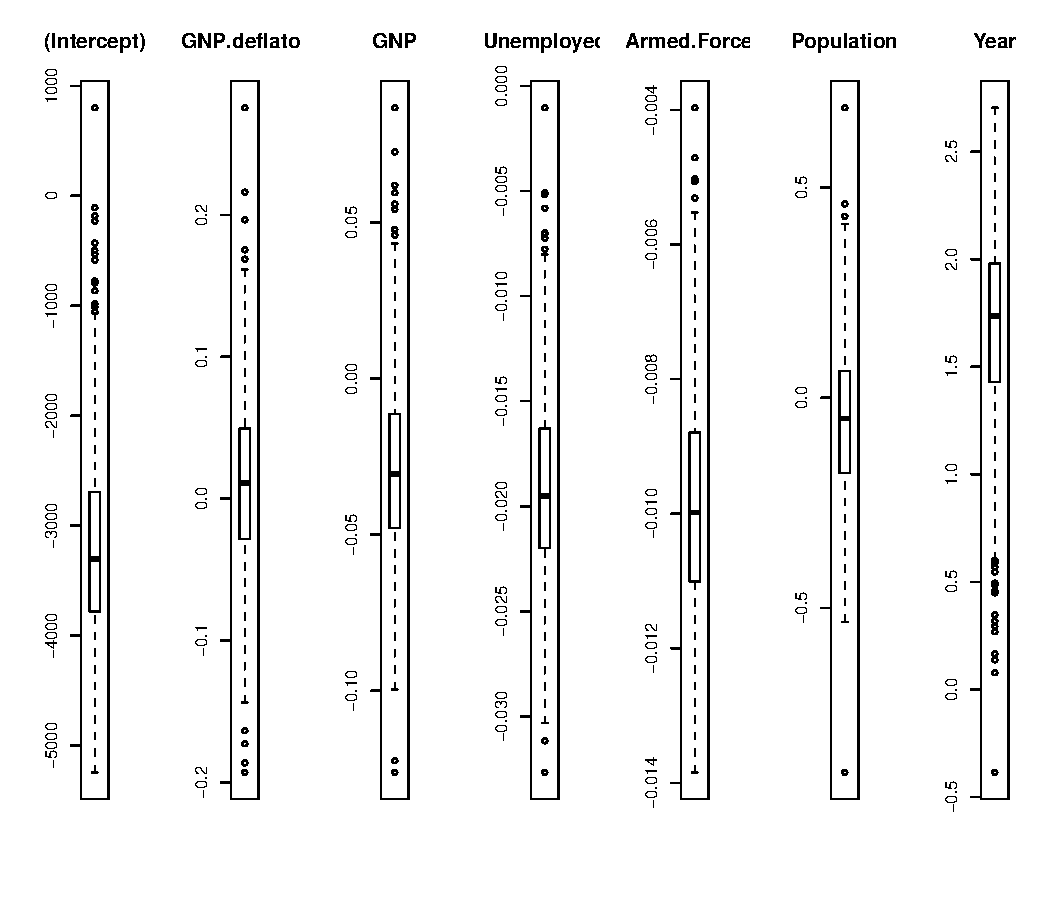
\includegraphics{accuracy_vignette-plot1a}
  \caption{\label{fig:plot1} Sensitivity Boxplots}
  \end{figure}

A tabular summary can reveal more information. The summary table compares the range of 
parameter estimates produced under perturbation to the original, unperturbed, parameter estimates. The table also highlights parameters that are particularly sensitive to perturbation -- the parameter estimate under perturbation exceeded the original estimate by more than +/- two times the original standard error in a disproportionate number of runs. For the Longley analysis, only some parameters are unstable:

\vbox{
\begin{Schunk}
\begin{Sinput}
R> print(summary(plongley), digits = 1)
\end{Sinput}
\begin{Soutput}
[1] "Sensitivity of coefficients over  500  perturbations:"
             Perturb Est. (Orig. Est.) (Orig. Stderr)   2.5%  97.5% [Unstable]
(Intercept)        -3e+03       -3e+03          9e+02 -5e+03 -1e+03          *
GNP.deflator        1e-02        2e-02          8e-02 -1e-01  1e-01           
GNP                -3e-02       -4e-02          3e-02 -8e-02  4e-02          *
Unemployed         -2e-02       -2e-02          5e-03 -3e-02 -8e-03          *
Armed.Forces       -1e-02       -1e-02          2e-03 -1e-02 -6e-03          *
Population         -7e-02       -5e-02          2e-01 -4e-01  3e-01           
Year                2e+00        2e+00          5e-01  6e-01  2e+00          *
\end{Soutput}
\end{Schunk}
}

In comparison, the ``Thurber'' example from the National Institute of Standards and Technology (NIST) statistical benchmark
datasets \citep{NIST98}, immediately below, exhibits instability in all parameters, while
the anorexia model following it is entirely insensitive to perturbation:

\vbox{
\begin{Schunk}
\begin{Sinput}
R> if (require("NISTnls", quietly = TRUE)) {
+     data("Thurber", package = "NISTnls")
+     fm1 <- nls(y ~ (b1 + x * (b2 + x * (b3 + b4 * x)))/(1 + x * 
+         (b5 + x * (b6 + x * b7))), data = Thurber, trace = FALSE, 
+         start = c(b1 = 1000, b2 = 1000, b3 = 400, b4 = 40, b5 = 0.7, 
+             b6 = 0.3, b7 = 0.03))
+     thurber.out <- sensitivity(Thurber, nls, y ~ (b1 + x * (b2 + 
+         x * (b3 + b4 * x))/(1 + x * (b5 + x * (b6 + x * b7)))), 
+         start <- c(b1 = 1000, b2 = 1000, b3 = 400, b4 = 40, b5 = 0.7, 
+             b6 = 0.3, b7 = 0.03))
+     print(summary(thurber.out), digits = 1)
+ }
\end{Sinput}
\begin{Soutput}
[1] "Sensitivity of coefficients over  50  perturbations:"
   Perturb Est. (Orig. Est.) (Orig. Stderr)   2.5% 97.5% [Unstable]
b1        1e+03        1e+03          5e+00  1e+03 1e+03           
b2        3e+02        2e+02          8e+00  2e+02 3e+02          *
b3        8e+01        7e+01          1e+01  7e+01 1e+02          *
b4        8e+00        1e+01          5e+00 -1e+01 1e+01          *
b5        1e+00        1e+00          3e-02  1e+00 1e+00          *
b6        4e-01        4e-01          1e-02  4e-01 5e-01          *
b7        6e-02        5e-02          7e-03  5e-02 1e-01          *
\end{Soutput}
\end{Schunk}
}
                          
                          

If error functions are not specified, a default set of error function will be 
selected based on the measurement type of each variable: continuous, ordered, or unordered.
Continuous variables, by default are subject to a small amount of
 mean-zero component-wise uniformly distributed
noise, which is typical of instrumentation-driven measurement error. Ordered factors
are assigned a small probability of having observations reclassified to the neighboring classification,
and unordered factors have a small probability of being reassigned to another legal value.

Alternatively, one can specify the error functions to use, or use one of many already available. 
The \pkg{accuracy} package comes with a wide range of functions to add noise to continuous variables 
and to randomly reclassify factor 
	variables.\footnote{The \pkg{perturb}  package for collinearity diagnosis by \citet{HenBelGrot04}(which was developed for \proglang{R} after the \pkg{accuracy} package) 
	provides additional methods for randomly reclassifying factors that via its 
	\code{reclassify()} function. This function can be used in conjunction with 
	\pkg{accuracy}. Hendrickx, et. al also provide a number of collinearity diagnostics, 
	including one based on data perturbations.} 

If measurement errors are correlated across variables, one can use a matrix-oriented
perturbation function, as illustrated below, returning to the Longley dataset:

\vbox{
\begin{Schunk}
\begin{Sinput}
R> if (require(MASS, quietly = TRUE)) {
+     plongleym <- sensitivity(longley, lm, Employed ~ ., ptb.rangen.ismatrix = TRUE, 
+         ptb.ran.gen = function(x, size = 1) {
+             mvrnorm(n = dim(x)[1], mu = rep(0, dim(x)[1]), Sigma = matrix(0.9, 
+                 nrow = dim(x)[1], ncol = dim(x)[1])) * size + 
+                 x
+         })
+ }
\end{Sinput}
\end{Schunk}
}

Your choice of error functions should reflect the measurement error model that is appropriate to the 
data you are using. In numerical analysis, uniform noise is often applied, since this is what would result from simple rounding error. Normal random noise is commonly used in statistics,
under the assumption that measurement error is the sum of multiple independent error processes. In 
addition, when normal perturbations are used, the result can be interpreted, for many models, as equivalent
to the results of running a slightly perturbed \emph{model} on unperturbed data. In some cases,
like discrete or ratio variables, other forms of noise are necessary to preserve
the structure of the problem. \citep[see, for example][section 16.3]{AltGilMcD03}. 
The magnitude of the noise is also under the control of the researcher. Most
choose a magnitude roughly proportionate to the researcher's qualitative estimate of the underlying measurement error in the data.
Noise is usually adjusted to the size of each component, since this better
preserves the structure of the problem, however in some cases the underlying
measurement error model may require norm-wise scaling of the noise. For more
information on noise distributions and measurement error models see , e.g., 
\citet{Belsley91,ChaiTrav04a,ChengVan99,Fuller87,CarRupStef95}.

We recommend that users run \code{sensitivity} multiple times with different noise specifications.
However, in our practical experience with social science analyses, the error model choice does not tend to affect the substantive conclusions from the sensitivity analysis.

Some researchers omit perturbations to outcome variables, since, in terms of
statistical theory, mean-zero measurement error on outcome variables (as opposed to explanatory variables)
contribute only to increased variance in estimates, not bias. While this attitude is justified 
in the context of statistical theory, it is not similarly justified in the computational realm. If the estimation
of a model is computationally unstable, errors in the outcome variable may have large and unpredictable
 biases on the model estimate. Hence, the conservative default in our package is to subject all variables to perturbation, although options are available to completely control the form and magnitude of all perturbations.

Consider this example, which shows a sensitivity analysis of the anorexia analysis described in \citet{VenRip02}. In this case, for 
	illustration,\footnote{In fact, applying the default perturbation to the dependent 
	variable affects this model only slightly.} 
we leave the dependent variable unperturbed, by assigning it the \emph{identity} error function.

\vbox{
\begin{Schunk}
\begin{Sinput}
R> data("anorexia", package = "MASS")
R> panorexia <- sensitivity(anorexia, glm, Postwt ~ Prewt + Treat + 
+     offset(Prewt), family = gaussian, ptb.R = 500, ptb.ran.gen = list(PTBi, 
+     PTBus, PTBus), ptb.s = c(1, 0.01, 0.01))
R> print(summary(panorexia), digits = 1)
\end{Sinput}
\begin{Soutput}
[1] "Sensitivity of coefficients over  500  perturbations:"
            Perturb Est. (Orig. Est.) (Orig. Stderr) 2.5% 97.5% [Unstable]
(Intercept)         49.8         49.8           13.4 48.3  51.3           
Prewt               -0.6         -0.6            0.2 -0.6  -0.5           
TreatCont           -4.1         -4.1            1.9 -4.2  -3.9           
TreatFT              4.6          4.6            2.1  4.4   4.7           
\end{Soutput}
\end{Schunk}
}

The anorexia example above is relatively stable. Most of the parameters estimates vary little over repeated perturbations.

Finally, if a \proglang{R} or \proglang{S-PLUS} model does not take a \code{data} argument or does not
return coefficients through the \code{coef} method, it is usually 
only a matter of a few minutes to write a
small wrapper that calls the original model with appropriate data, and that
provides a \code{coef} method for retrieving the results. (Alternatively, you
might to choose to run such models in \pkg{Zelig}, as described in the next section.)

For example, the \code{mle} function for maximum-likelihood estimation does
not have an explicit \code{data} option. Instead, it receives data implicitly
through the log-likelihood function, \code{ll}, passed into it. To adapt it for use
in \code{sensitivity} one simply constructs another function that accepts data and a 
log-likelihood function separately, constructs a temporary log-likelihood
function with the data passed in the environment, and then calls \code{mle}
with the temporary function:

\vbox{
\begin{Schunk}
\begin{Sinput}
R> mleD <- function(data, lld, ...) {
+     f <- formals(lld)
+     f[1] <- NULL
+     ll <- function() {
+         cl <- as.list(match.call())
+         cl[1] <- NULL
+         cl$data <- as.name("data")
+         do.call(lld, cl)
+     }
+     formals(ll) <- f
+     mle(ll, ...)
+ }
\end{Sinput}
\end{Schunk}
}

Finally, construct the log-likelihood function to accept data. As in this example, which
is based on the documented example in the \pkg{Stats4} package:

\vbox{
\begin{Schunk}
\begin{Sinput}
R> llD <- function(data, ymax = 15, xhalf = 6) -sum(stats::dpois(data[[2]], 
+     lambda = ymax/(1 + data[[1]]/xhalf), log = TRUE))
\end{Sinput}
\end{Schunk}
}

\subsection[Sensitivity Analysis of Zelig Models]{Sensitivity Analysis of \pkg{Zelig} Models}

\pkg{Zelig}\citep{Zelig07} is an \proglang{R} package that can estimate and help interpret
 the results of a large range of statistical models. \pkg{Zelig} provides
 a uniform interface to these models that \pkg{accuracy} 
utilizes to perform sensitivity analyses. In addition, \pkg{accuracy} can
also be used to perform sensitivity analyses of the robust alternatives, simulated 
predicted values, expected values, first differences, and risk ratios that \pkg{Zelig}
produces for all the models it 
	supports.\footnote{\pkg{Zelig} also integrates nonparametric matching methods as 
	an optional preprocessing step. Thus \pkg{accuracy} supports sensitivity analysis 
	of models subject to such pre-processing as well.}
So, using these packages together provides a convenient means to analyze the sensitivity 
of \emph{predicted values} to measurement error.


To illustrate, we replicate Longley's analysis, using
\code{zelig()} (instead of \code{lm}) to run the OLS model, and the convenience function
 \code{sensitivityZelig} to run the sensitivity analysis:

\vbox{
\begin{Schunk}
\begin{Sinput}
R> data(longley)
R> goodZelig <- require(Zelig, quietly = TRUE) && (!inherits(try(zelig(Employed ~ 
+     GNP, "ls", longley, cite = FALSE), silent = TRUE), "try-error"))
\end{Sinput}
\begin{Soutput}
## 
##  Zelig (Version 3.4-0, built: 2008-10-28)
##  Please refer to http://gking.harvard.edu/zelig for full documentation 
##  or help.zelig() for help with commands and models supported by Zelig.
##

##  Zelig project citations:
##    Kosuke Imai, Gary King, and Olivia Lau. 2005. ``Zelig: Everyone's
##    Statistical Software,'' http://gking.harvard.edu/zelig.
##  and
##    Kosuke Imai, Gary King, and Olivia Lau. 2009 (forthcoming). ``Toward A Common
##    Framework for Statistical Analysis and Development,'' Journal of Computational
##    and Graphical Statistics, http://gking.harvard.edu/files/abs/z-abs.shtml

##  To cite individual Zelig models, please use the citation format printed with
##  each model run and in the documentation.
##
\end{Soutput}
\begin{Sinput}
R> if (goodZelig) {
+     zelig.out <- zelig(Employed ~ GNP.deflator + GNP + Unemployed + 
+         Armed.Forces + Population + Year, "ls", longley)
+     perturb.zelig.out <- sensitivityZelig(zelig.out)
+ }
\end{Sinput}
\begin{Soutput}
How to cite this model in Zelig:
Kosuke Imai, Gary King, and Oliva Lau. 2007. "ls: Least Squares Regression for Continuous Dependent Variables" in Kosuke Imai, Gary King, and Olivia Lau, "Zelig: Everyone's Statistical Software," http://gking.harvard.edu/zelig
\end{Soutput}
\end{Schunk}
}

Just as above, \code{summary} and \code{plot(summary())} can be used summarize
the sensitivity of the model coefficients. In addition, we can use the 
\pkg{Zelig} methods \code{setx} and \code{sim} to simulate various
quantities of interest. And when \code{summary} and
 \code{plot} are used, they will display a \emph{sensitivity analysis} 
of the predicted values.

For example, the code below generates predictions of the distribution of the explanatory variable,
`Employed', around the point where `Year' equals 1955 
and the other variables are at their means, and creates a profile plot of 
the predicted distribution of the explanatory variable.

\begin{itemize}
\vbox{
\item  This sets the values of the explanatory variables to be used for the predictive simulation:
\begin{Schunk}
\begin{Sinput}
R> if (goodZelig) {
+     setx.out <- setx(perturb.zelig.out, Year = 1955)
+ }
\end{Sinput}
\end{Schunk}
}
\vbox{
\item  This performs the simulations, using the perturbed models: 
\begin{Schunk}
\begin{Sinput}
R> if (goodZelig) {
+     sim.perturb.zelig.out <- psim(perturb.zelig.out, setx.out)
+ }
\end{Sinput}
\end{Schunk}
}
\vbox{
\item This reports the range of predicted values, under perturbations. This can be thought of as predictions that are ``robust'' to perturbations, in an informal sense via a summary, and accompanying plot:
\begin{Schunk}
\begin{Sinput}
R> if (goodZelig) {
+     summary(sim.perturb.zelig.out)
+ }
\end{Sinput}
\begin{Soutput}
**** 50  COMBINED perturbation simulations 

  Model: ls 
  Number of simulations: 1000 

Values of X 
     (Intercept) GNP.deflator   GNP Unemployed Armed.Forces Population Year
1947           1        101.7 387.7      319.3        260.7      117.4 1954

Expected Values: E(Y|X)
      mean     sd  2.5% 97.5%
1947 65.31 0.1054 65.11 65.52
\end{Soutput}
\end{Schunk}
\begin{Schunk}
\begin{Sinput}
R> if (goodZelig) {
+     plot(sim.perturb.zelig.out)
+ } else {
+     plot(1, 1)
+ }
\end{Sinput}
\end{Schunk}
}
\end{itemize}

The resulting plot is shown in Figure~\ref{fig:plot2}.

\begin{figure}
\begin{Schunk}
\begin{Sinput}
R> if (goodZelig) {
+     plot(sim.perturb.zelig.out)
+ } else {
+     plot(1, 1)
+ }
\end{Sinput}
\begin{Soutput}
**** 50  COMBINED perturbation simulations 
\end{Soutput}
\end{Schunk}
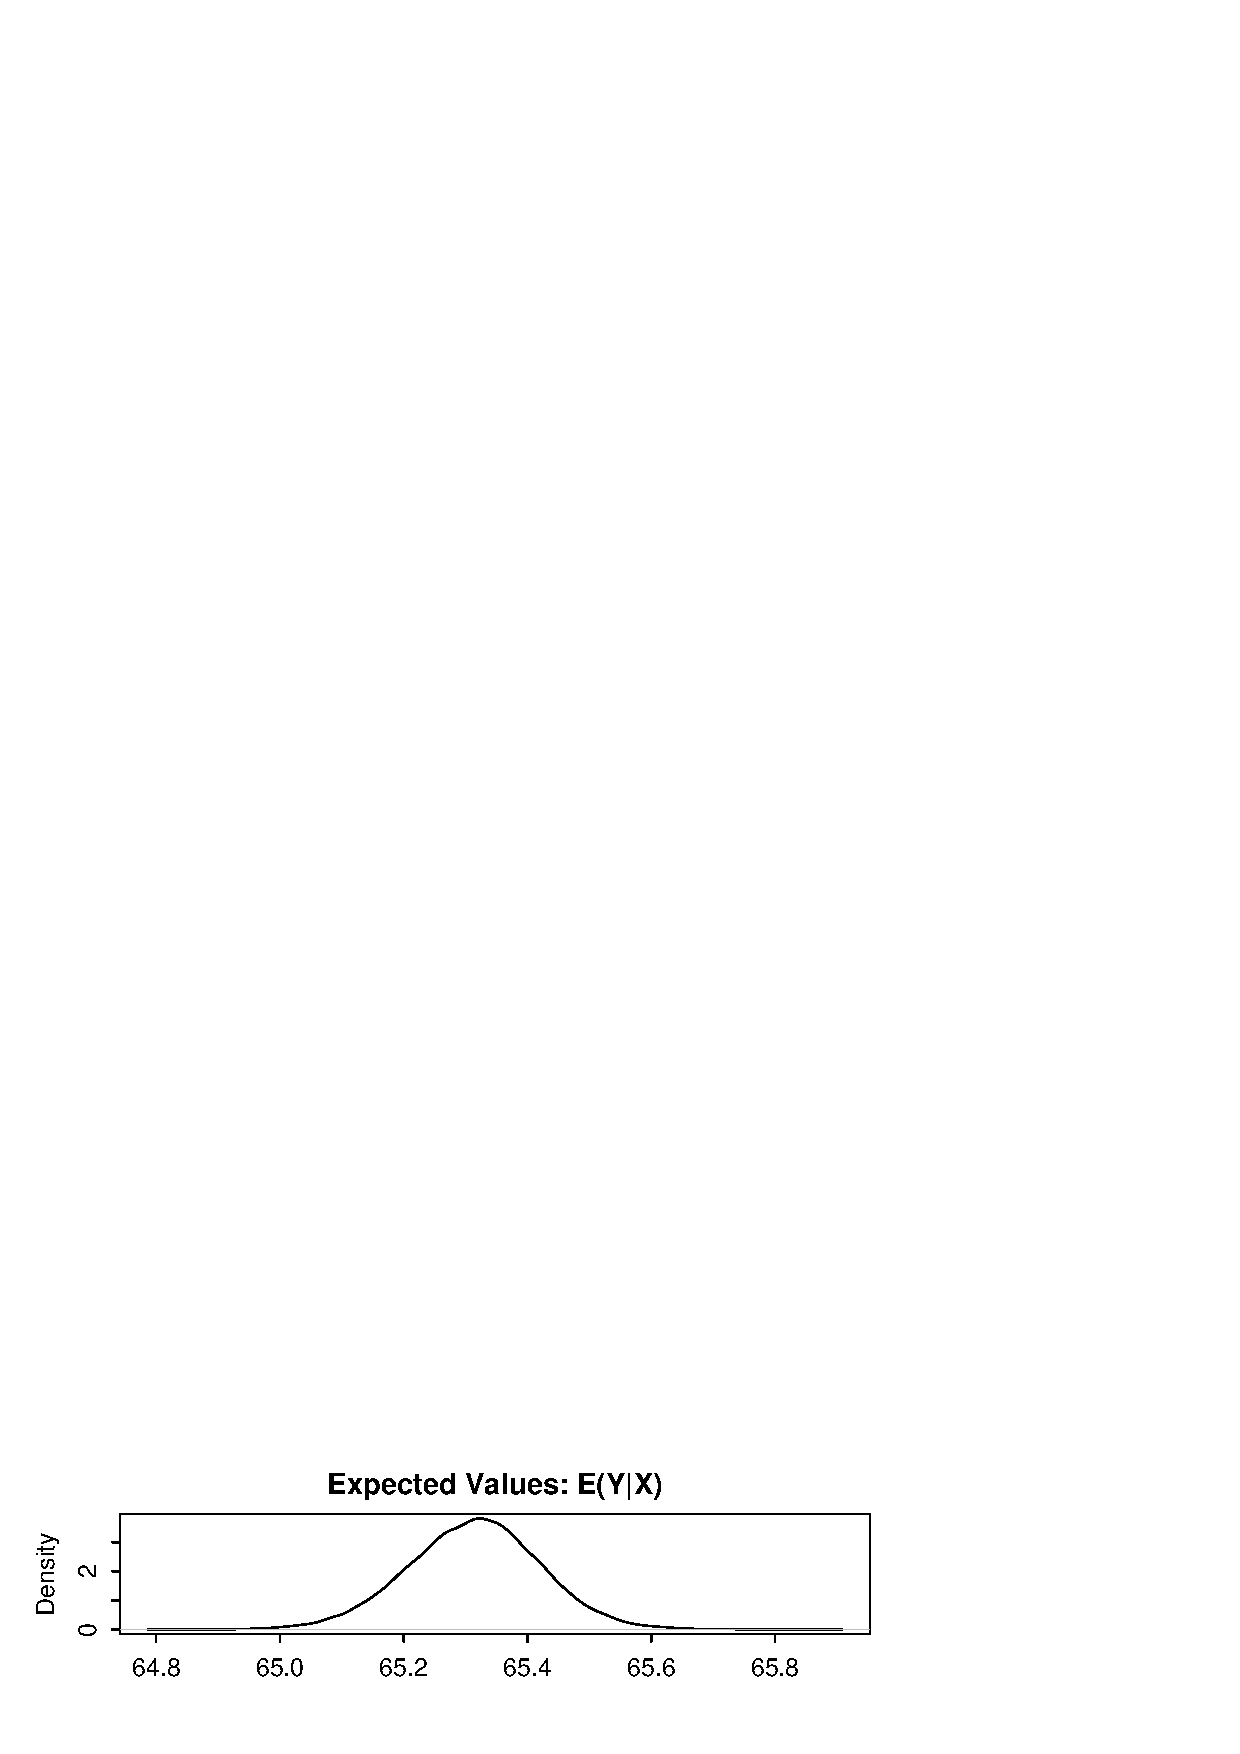
\includegraphics{accuracy_vignette-plot2a}
\caption{\label{fig:plot2} Posterior of dependent variable across perturbations}
\end{figure}


\section{More accurate computing} 

When a model is shown to be sensitive to perturbations, there are a number of possible culprits, including multiple optima, ill-conditioning, poor random number generation, and rounding error. Although there is no single tool that can identify or fix these root causes, \pkg{accuracy} offers a number of additional helpful tools for dealing with these sorts of issues. We discuss these in the following sections. 

\subsection{True random numbers through entropy collection}

`Random' numbers aren't. The numbers provided by routines such as \code{runif()} are not genuinely random.
 Instead, they are \emph{pseudo-random number generators}
(PRNG's), deterministic processes that create a sequence of numbers. 
Pseudo-random number generators start with a single ``seed'' value (specified by the user or based on a default value)
 and generate a repeating sequence with a certain
fixed length, or `period', $p$. This sequence is statistically
similar, in limited respects, to random draws from a uniform
distribution.

The earliest PRNG's, which are still in use in some places, and which were used in early versions of R, come 
from the family of Linear Congruential Generators (LCGs), defined 
	as:\footnote{All parameters are integers.}

\begin{align}\label{Congruential.Generator}
    LCG(a,m,s,c)&\equiv \nonumber\\
            x_{0} &=s,  \nonumber\\
            x_{n} &=(ax_{n-1}+c)\bmod{m}.
\end{align} 

This function generates a sequence of numbers between $[0,m-1]$ (in practice $x$ is usually divided by $m$ to yield numbers between zero and one) which appears to be, using some tests, uniformly distributed. Other PNRG's are more complex, but share with the LCG the fundamental properties of determinism and periodicity. See \cite{Gentle98} for an extensive treatment of modern PRNG's and theory.

\proglang{R} provides several high-quality PRNG's natively, and packages such as 
\pkg{gsl}, \pkg{rstream} and \pkg{rsprng} which can be used to generate
quasi-random number streams, and concurrent PRNG streams.
Regardless of the particular PRNG algorithm used, however, a PRNG cannot
perfectly mimic a random sequence. And, in fact, there is no complete
theory to describe the domains for which PRNG and true random sequences 
can be considered interchangeable. In addition, the theory
on which PRNG's are based assumes that the seed itself is \emph{truly} random.

The \code{runifT()} routine is different from other random number generators in R. 
It delivers true random numbers based on
entropy collected from external physical sources of randomness.

Three sources of randomness are currently supported. On Unix and Linux system, the kernel gathers environmental noise from 
device drivers and other sources into a system entropy pool.
This pool can be accessed through the `/dev/random' pseudo-device.
Alternatively, the ``Hotbits'' or ``random.org'' web-based
entropy servers, run by FourmiLab and the Distributed Systems Group
at Trinity college (respectively), provide random bytes collected from on physical noise sources.

Using any of these sources, \pkg{accuracy} retrieves chunks of random bits and stores them in a local pool for later use. This pool is used as necessary to 
 satisfy calls to \code{runifT()} and \code{resetSeed()},
 and is automatically refreshed from the external sources when empty. 
 If external sources are unavailable, the pool is refreshed using standard PRNG's.

Entropy collection is relatively slow compared to PRNG's. So, these routines
are most practical for generating either small numbers of very high quality random
numbers (e.g. for cryptography) or for seeding (and regularly reseeding) PRNG's. 
The function \code{resetSeed()} sets the seed for the standard PRNG\'s using
true random bits. The \code{runifS()} automates this process further, by reseeding 
runif() with random values, periodically, to improve the random properties of the
 resulting sequence:

\vbox{
For illustration we implement a test of randomness \citep{MarTsa02}:
\begin{Schunk}
\begin{Sinput}
R> birthday <- function(x, n = 2^20) {
+     spacings <- diff(trunc((x * .Machine$integer.max)%%n))
+     tab <- table(spacings)
+     tab <- tab[which(tab > 1)]
+     chisq.test(sample(tab, 200, replace = T))
+ }
\end{Sinput}
\end{Schunk}
}

\vbox{
This randomly resets the seed used by default PRNG:

\begin{Schunk}
\begin{Sinput}
R> old.seed <- resetSeed()
R> y = runif(1e+06)
R> birthday(y)
\end{Sinput}
\begin{Soutput}
	Chi-squared test for given probabilities

data:  sample(tab, 200, replace = T) 
X-squared = 22.89, df = 199, p-value = 1
\end{Soutput}
\end{Schunk}
}

\vbox{
Alternately, this resets the seed for the PRNG's after every 10000 draws:
   
\begin{Schunk}
\begin{Sinput}
R> y <- runifS(1e+06)
R> birthday(y)
\end{Sinput}
\begin{Soutput}
	Chi-squared test for given probabilities

data:  sample(tab, 200, replace = T) 
X-squared = 22.65, df = 199, p-value = 1
\end{Soutput}
\end{Schunk}
} 

For most applications, researchers using PRNG's should simply substitute \code{runifS} in for \code{runif}. For cryptographic applications, using \code{runifT} is appropriate. 

\subsection{Tests for global optimality}

The estimation of many statistical models rests on finding the global optimum
to a user-specified non-linear function. R provides a number of tools for such
estimations, including \code{nlm()}, \code{nls()}, \code{mle()}, 
\code{optim()} and \code{constrOptim()}. 

All of these functions rely on local search algorithms, and the results they
return may depend on the starting point of the search. Maximum likelihood functions, non-linear-regression models, and the like, are not guaranteed to 
be globally convex in general. And even where convexity is guaranteed by statistical theory, inaccuracies in statistical computation can sometimes induce false local optima (discontinuities that may cause local search algorithms to converge, or at least stop). A poor or unlucky choice of starting values may cause a search algorithm to converge at a local optimum, which may be far from the real global optimum of the function. Inferences based on the values of the parameters at the local optimum will not be correct. 

Knowing when a function has reached its true maximum is
something of an art. While the plausibility of the solution
in substantive terms is often used as a check, relying solely on the expected
answer as a diagnostic might bias researchers toward Type I errors, rejecting the null hypothesis when it is true. Diagnostic
tests are therefore useful to provide evidence that the computed
solution is the true solution. If such tests indicate that the global optimum has not been reached, the user may consider a closer examination of starting values, applying an alternative optimization algorithm, and/or heuristic designed for non-smooth optimization problems, such as the simulated annealing option for \code{optim()}, or the optimizers provided by the \pkg{gafit} \citep{gafit02}, \pkg{genalg} \citep{genalg05}, \pkg{rgenoud}  \citep{rgenoud07} modules.

A number of strategies related to the choice of starting values have been formalized as tests 
or global optimality. In this package we implement two. The `Starr' test and the `Dehaan' 
	test.\footnote{In addition to these tests, the \proglang{R} user may also wish to 
	investigate the \pkg{Bhat} \citep{bhat05} package, which can generate diagnostic profile likelihood 
	plots.} 
 
The intuition behind the Starr test statistic is to run the optimization from 
different starting points to observe `basins of attraction', and then to
estimate the number of \emph{unobserved} basins of attraction from the
number of observed basins of attraction. The greater the number
of observed basins of attraction, the lower the probability that a
global optimum has been located. This idea has been attributed to \citet{Turing48},
and the test statistics was developed by \citet{Starr79}:
\begin{equation}\label{Starr.test.equation}
    V_{2}=\frac{S}{r}+\frac{2D}{r\left( r-1\right)}.
\end{equation} Here $V_2$ is the probability a convergence
point has not been observed, and $r$ is the number of randomly
chosen starting points. $S$ is the number of convergence points
that were produced from one (or a {\underline{S}}ingle) starting
value and $D$ is the number of convergence points that were
produced from two (or {\underline{D}}ouble) different starting
values. 

\citet{FinMenTho89} demonstrate the value of the
statistic by analyzing a one parameter equation on a $[0,1]$
interval for $r = 100$. While the proposed statistic given by the
above equation is compelling, their example is similar to an
exhaustive grid search on the $[0,1]$ interval. 
(Starr's result is further generalizable for triples and
higher order observed clumping of starting values into their
basins of attraction, but Finch, Mendell, and Thode assert that
counting the number of singles and doubles is usually sufficient.)

The statistic may be infeasible to compute for an unbounded parameter space with 
high dimensionality. However, the intuition behind the statistic
can still be applied soundly in these cases. If multiple local optima are identified over the
course of a search for good starting values, a researcher should
not simply stop once an apparent best fit has been found,
especially if there are a number of local optima which have basins
of attraction that were identified only once or twice. Our implementation
of the Starr test provides a ready-to-use-interface that can be 
easily incorporated into a search of the parameter space for good optimization 
starting values.

For computationally intensive problems, another test, proposed by \citet{Veall90}, drawing upon a 
result presented by \citet{deHaan81}, may be more practical. The de Haan/Veall test relies on
 sampling the optimization function itself rather than
identifying basins of attraction. A confidence interval for 
the value of the likelihood function's global optimum is generated from
the points sampled from the likelihood surface. This procedure is much faster than the Starr
test because the likelihood function is calculated only once for each 
trial, as opposed to running the optimization algorithm many times to identify basins of attraction. As with starting value searches, researchers are
advised to increase the bounds of the search area and the number
of trials if the function to be evaluated has a high degree of
dimensionality or a high number of local optima have been
identified.

Veall suggests that by using a random search and applying extreme asymptotic theory, a confidence interval for the candidate
solution can be formulated. The method, according to Veall (pg. 
1460) is to randomly choose a large number, $n$, of values for the
parameter vector using a uniform density over the entire parameter
space. Call the largest value of the evaluated likelihood function
$L_1$ and the second largest value $L_2$. The $1-p$ confidence
interval for the candidate solution, $L^{'}$, is $[L_1,L^p]$
where:

\begin{equation}\label{Veall.test.equation}
    L^p =L_1+\frac{ L_1-L_2 }{ p^{-1/\alpha}-1 }
\end{equation}
and $\alpha = k/2$, where $k$ is some function that depends on $n$ such that
$k(n)/n\rightarrow 0$, as $k(n),n \rightarrow \infty$ (a likely candidate is
$k=\sqrt{n}$).

As Veall (pg. 1461) notes, the bounds on the search of the
parameter space must be large enough to capture the global maximum
and $n$ must be large enough to apply asymptotic theory. In Monte
Carlo simulations, Veall suggests that 500 trials are sufficient
for rejecting that a local optimum is not the \emph{a priori}
identified global optimum. 

\vbox{
Examples of applying both the Dehaan and Starr tests are below:
\begin{Schunk}
\begin{Sinput}
R> data("BOD")
R> stval <- expand.grid(A = seq(10, 100, 2), lrc = seq(0.5, 0.8, 
+     0.025))
R> stval <- stval + cbind(runif(dim(stval)[1]), runif(dim(stval)[1]) * 
+     0.01)
R> llfun <- function(A, lrc) -sum((BOD$demand - A * (1 - exp(-exp(lrc) * 
+     BOD$Time)))^2)
R> lls <- NULL
R> for (i in 1:nrow(stval)) {
+     lls <- rbind(lls, llfun(stval[i, 1], stval[i, 2]))
+ }
R> fm1 <- nls(demand ~ A * (1 - exp(-exp(lrc) * Time)), data = BOD, 
+     start = c(A = 20, lrc = log(0.35)))
R> ss <- -sum(resid(fm1)^2)
R> dehaan(lls, ss)
\end{Sinput}
\begin{Soutput}
[1] TRUE
\end{Soutput}
\end{Schunk}
}

\vbox{
\begin{Schunk}
\begin{Sinput}
R> llb <- NULL
R> for (i in 1:nrow(stval)) {
+     llb <- rbind(llb, coef(nls(demand ~ A * (1 - exp(-exp(lrc) * 
+         Time)), data = BOD, start = c(A = stval[i, 1], lrc = stval[i, 
+         2]))))
+ }
R> starr(llb)
\end{Sinput}
\begin{Soutput}
[1] 0
\end{Soutput}
\end{Schunk}
}

In the examples above, both tests report positive results. 
The researcher can thus be more confident that \code{nls} has converged to the global optimum. In the next section we examine the case where the estimation of a model
has converged, but yields a Hessian that cannot be inverted.
 
\subsection{A generalized Cholesky method}

We include in the \pkg{accuracy} package is an implementation of the \citet{SchEsk90} matrix
Cholesky decomposition algorithm as implemented in \citet{GilKin04}. Essentially this asks the question, 
if my Hessian (or any other matrix) cannot be decomposed by the Cholesky algorithm for low-level numerical 
reasons (or perhaps other reasons), then what is the smallest amount I need to change the matrix to make 
it decomposable. Recall that the Cholesky decomposition is defined as $\mathbf{V}$ in the decomposition 
$\mathbf{C} = \mathbf{V}'\mathbf{V}$ for the matrix $\mathbf{C}$. Of course this idea of ``change'' has 
for the algorithm multidimensional consequences and the elegance of the Schnabel and Eskow approach is that 
takes this into account over the more primitive solutions whereby changes can impose greater consequences
down the procedure \citep{GilMur74}. Their method, based on Gerschgorin bounds, is implemented in our
function \code{sechol}.

The generalized inverse is a commonly used technique
in statistical analysis, but the generalized Cholesky has not, to our knowlesge, before
been used for statistical purposes, prior to its appearance in Altman, Gill, \& McDonald 2003. When the inverse of the negative Hessian does not exist, we suggest
the following procedure: Create a
\emph{pseudo-variance matrix} and use it, in place of the inverse, in
an importance resampling scheme.
In brief, applying a generalized inverse (when necessary, to avoid singularity) and generalized
Cholesky decomposition (when necessary, to guarantee positive
definiteness) together often produce a pseudo-variance matrix for the
mode that is a reasonable summary of the curvature of the posterior
distribution. This method is developed and analyzed in detail in \citet{GilKin04},
here we provide a brief sketch.

The Gill/Murray Cholesky factorization of a singular matrix C, adds 
a diagonal matrix E such that the standard Cholesky procedure is defined. 
Unfortunately it often increments C by an amount much larger than necessary, providing 
a pseudo-Cholesky result that is further away from the intended result. 
\citet{SchEsk90} improve on the C+E procedure of Gill and Murray by
applying the Gerschgorin Circle Theorem to reduce the infinity norm of the E matrix. The strategy is to calculate
delta values that reduce the \emph{overall} difference between the singular matrix and
the incremented matrix. This improves the Gill/Murray approach of incrementing diagonal
values of a singular matrix sufficiently that Cholesky steps can be performed.

This technique is complex to describe but simple to use. The following is an example of its use
with a singular matrix:

\vbox{
\begin{Schunk}
\begin{Sinput}
R> S <- matrix(c(2, 0, 2.5, 0, 2, 0, 2.5, 0, 3), ncol = 3)
R> sechol(S)
\end{Sinput}
\begin{Soutput}
      [,1]  [,2]     [,3]
[1,] 1.414 0.000 1.767767
[2,] 0.000 1.414 0.000000
[3,] 0.000 0.000 0.004262
attr(,"delta")
[1] 1.817e-05
\end{Soutput}
\end{Schunk}
}

Surprisingly, the matrix resulting from the generalized inverse and Cholesky combination
 is not usually ill-conditioned. In addition,
although this is a ``pseudo'' rather than ``approximate'' variance
matrix (because the approximated matrix does not exist),
the calculations make only small changes in the resulting variance matrix to achieve positive definiteness. We then take random draws
from the exact posterior using importance resampling, but
recommend two diagnostics to correct potential problems with this procedure. 

A diagnostic often used to detect a failure of importance resampling is a high rejection rate of 
candidate values of $\tilde{\boldsymbol{\theta}}$, often due to low values of
the importance ratio. In this case the procedure will run for a long time, and even though the procedure may eventually yield sufficient sample
size, this can be very frustrating and time-consuming. However, a long run time may warn that the approximation distribution 
fails to capture a range of values of $\boldsymbol{\theta}$ that have posterior density
systematically different from the rest. Since the normal has support over
$(-\infty,\infty)$, the potential for this problem to occur vanishes as the number of
simulations grows. Therefore another diagnostic check computes a very large number of simulations
with an artificially large variance matrix, such as the pseudo-variance matrix multiplied
by a positive factor, which we label $F$. The more diffuse coverage can identify missed values, however, like all related simulation procedures, it is impossible to cover the full
continuum of values that $\boldsymbol{\theta}$ can take, and the procedure can miss
subtle features like pinholes in the surface, very sharp ridges, or other eccentricities. Similar to our examination of likelihood maximia, the 
difficulty in identifying such features is most pronounced for complex, multi-dimensional problems.

\subsubsection{Uninvertible Hessian matrices}

As an example, consider the effect of \code{sechol} on the progressively ill-conditioned matrices below.

\vbox{
\begin{itemize}
\item This matrix is invertible, so both \code{sechol} yields the same results as \code{chol}:
\begin{Schunk}
\begin{Sinput}
R> S <- matrix(c(2, 0, 2.4, 0, 2, 0, 2.4, 0, 3), ncol = 3)
R> print(try(chol(S)))
\end{Sinput}
\begin{Soutput}
      [,1]  [,2]   [,3]
[1,] 1.414 0.000 1.6971
[2,] 0.000 1.414 0.0000
[3,] 0.000 0.000 0.3464
\end{Soutput}
\begin{Sinput}
R> sechol.out <- sechol(S)
R> t(sechol.out) %*% sechol.out
\end{Sinput}
\begin{Soutput}
     [,1] [,2] [,3]
[1,]  2.0    0  2.4
[2,]  0.0    2  0.0
[3,]  2.4    0  3.0
\end{Soutput}
\end{Schunk}

\item This matrix is not invertible, so \code{sechol} works, and \code{chol} does not
\begin{Schunk}
\begin{Sinput}
R> S <- matrix(c(2, 0, 10, 0, 2, 0, 10, 0, 3), ncol = 3)
R> print(try(chol(S)))
\end{Sinput}
\begin{Soutput}
[1] "Error in chol.default(S) : \n  the leading minor of order 3 is not positive definite\n"
attr(,"class")
[1] "try-error"
\end{Soutput}
\begin{Sinput}
R> sechol.out <- sechol(S)
R> t(sechol.out) %*% sechol.out
\end{Sinput}
\begin{Soutput}
     [,1] [,2] [,3]
[1,]    2    0   10
[2,]    0    2    0
[3,]   10    0   50
\end{Soutput}
\end{Schunk}
\end{itemize}
}

It should be clear that the meaning of `works', as above, depends greatly on the extent of the singularity in
the matrix. More generally, consider the example from \citet{AltGilMcD03}:
\begin{equation}\label{sechol1.example}
  	\text{Var}Sigma_1=\left[\begin{matrix} 2 & 0 & 2.4\\ 0 & 2 & 0\\ 2.4 & 0 & 3 \end{matrix}\right].
\end{equation}
The Cholesky decomposition of this matrix is given by:
\begin{equation}
        \text{chol}(\text{Var}Sigma_1) = \left[ \begin{matrix} 1.41 & 0 & 1.69\\ 0
	& 1.41 & 0\\ 0 & 0 & 0.35 \end{matrix} \right].
\end{equation}
The procedure works since this matrix is positive definite. Suppose now that we change the values on 
the corners have been changed from $2.4$ to $2.5$. Now the matrix is nonpositive definite and we
cannot calculate the Cholesky decomposition in the normal manner. However, \code{sechol} returns
\begin{equation}
  	\text{GCHOL}(\text{Var}Sigma_2)=\left[ \begin{matrix} 1.58 & 0 & 1.58\\ 0
        & 1.41 & 0\\ 0 & 0 & 0.71 \end{matrix} \right],
\end{equation}
which preserves the sense that only a small change ($2.4$ to $2.5$) has been made.

\subsubsection{Example: prior elicitation for logit regression}

Bayesian applications of the logit model for dichotomous outcomes are quite common and often 
use rather vague priors. Suppose, instead, that we want to elicit prior information from 
subject matter experts and include this explicitly qualitative information in the statistical 
model. In this way the Bayesian posterior 
distribution is a compromise between expert knowledge and the data at hand. Arguments for 
this approach can be found in \citet{GilWal05}.

Begin with the basic logit regression model conforming to the standard assumptions, defining terms conventionally: 
\begin{equation}
  P(\mathbf{Y}_i=1|\mathbf{X})=[1+\exp(\mathbf{X}_i\boldsymbol{\theta})]^{-1}
\end{equation}
, where $\mathbf{X}$ is an $n \times p$, rank $p$ matrix of explanatory variables with a leading column of 
 ones for the constant, $\boldsymbol{\theta}$  is a $p \times 1$ vector of coefficients,
  $\mathbf{Y}$ is an $n \times 1$ vector of observed outcome 
variable values, and $\boldsymbol{\epsilon}$ is a $n \times 1$ vector of errors. The Bayesian approach to 
uninformed priors for this model often specifies that $p(\boldsymbol{\theta}) \propto c$ over 
$(-\infty,\infty)$ for an arbitrary constant value $c$. 

To elicit prior judgments for the prior, experts need to be queried in such a way 
some parametric form for the prior on $\boldsymbol{\theta}$ can be stipulated that conforms to their 
assessments. \citet{KadDicWin80} suggest the following approach: Establish $j$ design 
points of the explanatory variable vector, $\tilde{\mathbf{X}}_1,\tilde{\mathbf{X}}_2,\ldots,\tilde{\mathbf{X}}_j$,
such that these represent interesting cases spanning the range of the $p$ variables.
The assessors are asked to study each of the $\tilde{\mathbf{X}}_i$ scenarios and produce $\mathbf{Y}^*_i$, 
an expected outcome variable (zero or one) corresponding to the design point cases. Such a 
value represents a typical response to the hypothesized design point, $\tilde{\mathbf{X}}_i$. For a 
single expert, the result is a ``stacked'' design matrix from collecting the $\tilde{\mathbf{X}}_i$ 
values, and an expected outcome variable vector from collecting the $\mathbf{Y}_i$ values. 

An elicited prior point estimate for $\boldsymbol{\boldsymbol{\theta}}$ is produced by running a logit model
as if these were conventional data. However, if the researcher does not 
ensure that the design matrix leads to a positive definite Hessian matrix (the matrix of second
derivatives at the MLE point estimates) in the estimation process, then she may proceed to elicit responses 
from the expert before noticing that the Hessian cannot produce a variance/covariance matrix for 
the estimated coefficients (there is nothing in the definition of 
interesting $\tilde{\mathbf{X}}_i$ cases that ensures this). Since these experts are often busy and difficult to schedule, 
repeating the process may not be possible. Obviously, the matrix can be reconfigured by 
deleting cases, but this leads to a loss of information and potential biases. 

Consider the following simple case from education policy. The \textsf{California Department of Education} (CDE) collected testing data 
for unified school districts and collections of schools that logically constitute similar
units ($n=303$) in 1998 by requiring students in the $2^{\text{nd}}$ through $11^{\text{th}}$ grade to take standardized tests for 
a variety of subjects including mathematics, which we will analyze here, at each grade level (the 
Stanford 9). The raw test scores are replaced with a binary outcome indicating whether or not 
the student exceeded the national median, summed by district, as a way to deal with large
measurement error (this is also a criteria for evaluating administrators). The following 
design matrix (with insufficient variation) is stipulated:

\begin{equation*}
    \mathbf{X}' = \left[ \begin{array}{lrrrrrrrr}
	Percent Low Income       &  10&  30&  25&  55&  50&  40&  30&  15 \\
	Mean Teacher Experience  &   5&  30&  15&  10&  17&  15&  15&  22 \\
	Per-Pupil Spending       &5002&5000&5000&5000&5000&5000&5000&5000 \\
	Percent Minority Teachers&  21&  22&  22&  22&  22&  22&  22&  21 \\
	Class Size               &  20&  20&  21&  22&  18&  20&  24&  18 \\
    \end{array} \right].
\end{equation*}
% code for data matrix above, initialize but don't show
Elicitations are produced by an expert in education policy, giving the following vector:
$\mathbf{Y} = [1,0,0,0,1,1,0,1]$ (test scores are heavily influenced by demographics in this policy
environment). These numbers are admittedly synthetic but are contrived to show how easy the
following problem emerges. 


\vbox{
Running a standard probit model through \code{glm} produces a warning and nonsensical 
estimates:
\begin{Schunk}
\begin{Sinput}
R> glm(Y.vec ~ X.mat[, -1], family = binomial(link = "probit"))
\end{Sinput}
\begin{Soutput}
Call:  glm(formula = Y.vec ~ X.mat[, -1], family = binomial(link = "probit")) 

Coefficients:
                         (Intercept)         X.mat[, -1]Percent Low Income  
                           -2.04e+04                              2.03e-01  
  X.mat[, -1]Mean Teacher Experience         X.mat[, -1]Per-Pupil Spending  
                           -7.42e-01                              4.07e+00  
X.mat[, -1]Percent Minority Teachers                 X.mat[, -1]Class Size  
                            9.05e+00                             -9.87e+00  

Degrees of Freedom: 7 Total (i.e. Null);  2 Residual
Null Deviance:	    11.1 
Residual Deviance: 3e-10 	AIC: 12 
\end{Soutput}
\end{Schunk}
}
\vbox{
One gets somewhat farther constucting the probit likelihood and using \code{optim}:

\begin{Schunk}
\begin{Sinput}
R> probit.log.like <- function(beta, X, Y) {
+     -sum(log(1 - pnorm(X %*% beta)) * (1 - Y)) - sum(log(pnorm(X %*% 
+         beta)) * Y)
+ }
R> dd.log.like <- function(beta, X, Y) {
+     lambda.0 <- (1 - Y) * (-1 * dnorm(X %*% beta)/(1 - pnorm(X %*% 
+         beta)))
+     lambda.1 <- Y * dnorm(X %*% beta)/(pnorm(X %*% beta))
+     (-sum(lambda.0 * (lambda.0 + X %*% beta) * (1 - Y)) * t(X) %*% 
+         X - sum(lambda.1 * (lambda.1 + X %*% beta) * (Y)) * t(X) %*% 
+         X)
+ }
R> star.prob <- optim(fn = probit.log.like, par = rep(0, ncol(X.mat)), 
+     X = X.mat, Y = Y.vec)
R> star.pars = star.prob$par
R> names(star.pars) = dimnames(X.mat)[[2]]
R> star.pars
\end{Sinput}
\begin{Soutput}
                 Constant        Percent Low Income   Mean Teacher Experience 
                  1.55672                   0.03890                  -0.34391 
       Per-Pupil Spending Percent Minority Teachers                Class Size 
                  0.01009                   0.99277                  -3.42488 
\end{Soutput}
\end{Schunk}
}

\vbox{
However, the resulting Hessian matrix is singular and cannot be inverted: 

\begin{Schunk}
\begin{Sinput}
R> star.hess <- dd.log.like(star.prob$par, X.mat, Y.vec)
R> matrix(star.hess, nrow = 6)
\end{Sinput}
\begin{Soutput}
           [,1]       [,2]       [,3]      [,4]       [,5]       [,6]
[1,]     -2.189     -69.79     -35.31    -10948     -47.62     -44.61
[2,]    -69.790   -2702.65   -1123.48   -348955   -1528.53   -1430.01
[3,]    -35.305   -1123.48    -676.82   -176530    -769.33    -710.76
[4,] -10947.973 -348954.67 -176529.98 -54742603 -238118.00 -223064.75
[5,]    -47.621   -1528.53    -769.33   -238118   -1036.17    -971.04
[6,]    -44.611   -1430.01    -710.76   -223065    -971.04    -916.57
\end{Soutput}
\begin{Sinput}
R> strsplit(try(solve(star.hess)), ":")
\end{Sinput}
\begin{Soutput}
[[1]]
[1] "Error in solve.default(star.hess) "          
[2] " \n  system is computationally singular"     
[3] " reciprocal condition number = 1.93887e-16\n"
\end{Soutput}
\end{Schunk}
}

\vbox{
Using the Moore-Penrose generalized inverse we can produce a serviceable variance/covariance 
matrix but it is not positive definite and we cannot therefore apply the Cholesky decomposition 
to get usable standard errors:
\begin{Schunk}
\begin{Sinput}
R> library("MASS")
R> star.vc <- ginv(-star.hess)
R> strsplit(try(chol(star.vc)), ":")
\end{Sinput}
\begin{Soutput}
[[1]]
[1] "Error in chol.default(star.vc) "                             
[2] " \n  the leading minor of order 5 is not positive definite\n"
\end{Soutput}
\end{Schunk}
}

\vbox{
Fortunately the Schnabel and Eskow variant of the Cholesky 
decomposition (implemented and discussed in \citet{GilKin04}) is able to do this:
\begin{Schunk}
\begin{Sinput}
R> round(sechol(star.vc), 4)
\end{Sinput}
\begin{Soutput}
     [,1]    [,2]   [,3]    [,4]    [,5]    [,6]
[1,]    0 -0.0057 0.0486 -0.0018  0.0392  0.3707
[2,]    0  0.0459 0.0020 -0.0002 -0.0004 -0.0137
[3,]    0  0.0000 0.0883  0.0001 -0.0060 -0.0772
[4,]    0  0.0000 0.0000  0.0001 -0.0002 -0.0020
[5,]    0  0.0000 0.0000  0.0000  0.0009  0.0000
[6,]    0  0.0000 0.0000  0.0000  0.0000  0.0010
attr(,"delta")
[1] 8.695e-07
\end{Soutput}
\end{Schunk}
}

Obviously this highlights a severe problem (i.e., the first column), but it gives useful
information for the other dimensions. Since the first column is for the constant, we can
replace zero with an arbitrary positive standard error in the prior assignment (for instance,
from a modified problem) without causing much controversy. 

So now we have plausible standard errors for all terms but the constant, without having to 
re-specify the model completely:
\begin{equation}
  SE = [0.0459, 0.0883, 0.0001, 0.0009, 0.0009]
\end{equation}
 In this case the glm function in R 
provided results but with a warning that the fitted values are very close
to zero or one where it is very difficult (numerically) to get measures
of curvature. This is because the right-hand-side of the GLM 
specification is very large in absolute value pushing way into the probit
function as it asymptotically approaches the limit. As such, a 
conventional estimation does not exist since it is not possible perfectly
separate the two possible outcomes \citep{VenRip02}.

This estimation
process is not the actual Bayesian production of a posterior, but is designed to extract
qualitative information into a prior specification. From here, the researcher may impose
a parametric assumption (normal, t, etc.) and use these values, or may engage in the more
involved process of stipulating something nonparametric.


\section{Obtaining the software}

In this article, we have discussed a number of tools and methods for assessing the sensitivity of 
complex models to numerical and measurement error. These tools are all included in the \pkg{accuracy}
 module, which can be obtained from any CRAN mirror (\url{http://cran.r-project.org/}), from
the new CSAN site {\url{http://csan.insightful.com}), 
or from our website: 
	\url{http://www.hmdc.harvard.edu/micah_altman/software}.\footnote{We also maintain a catalog 
	of links to other tools for computationally accurate statistics here: 
	\url{http://www.hmdc.harvard.edu/numal/resources/}.} 

\pkg{accuracy} (with \pkg{Zelig}) has also been incorporated in the \textbf{Virtual Data Center} (VDC) 
\citep{AltAndDig01} digital library and data analysis system. This offers a web-based interface to 
perform simulation and sensitivity analysis that is simple enough for even novices to use. The VDC 
system is available from: \url{http://thedata.org}.
 
\section{Acknowledgements}\vspace{-5pt}
We thank John Chambers, Kurt Hornik, Gary King, Eduardo Leoni, and Duncan Murdoch for their comments on the software and article.
%%\renewcommand{\baselinestretch}{1}

\bibliographystyle{unsrtnat}

\bibliography{jstatsoft_acc}
\end{document}
